\chapter{建構黑洞與近視界之謎}

\lectureoverview{我們將用三個部分來建構黑洞：平直時空的因果圖、史瓦西圖，以及球殼的伯克霍夫定理。這個建構揭示，事件視界是一道全域邊界，而且可以從局部仍然平直的區域開始。接著，我們從因果幾何轉向熵與霍金溫度。放在視界附近的溫度計會變得任意熱，但自由落下的觀測者預期不會遭遇局部災難。最後的論證追問：外部實驗究竟能確立什麼，又如何避免製造出它原本要探測的擾動？}

\section{溫度與空無一物的空間相同的黑洞}

原本應該有份作業：建構一個黑洞，帶到課堂上展示講解。沒有人能拿出黑洞展示，但透過 Wolfram 找到的一項計算，提供了一個比較簡單的開場問題。要讓黑洞的霍金溫度接近宇宙微波背景的 \(3\,\mathrm{K}\) 溫度，它的半徑和質量應該是多少？

\begin{classroomqa}
\audiencequestion{網站上算的是什麼？\lecturetimestamp{00:00:39}}
\lecturerresponse{溫度約為 \(3\,\mathrm{K}\) 的黑洞，其半徑是多少。重點不在精確計算，而在估計物理尺度。}
\end{classroomqa}

這樣的黑洞會短暫地與周遭環境同溫，但這種平衡並不穩定。史瓦西黑洞的熱容為負。若它比熱浴稍熱，就會放出輻射、失去質量，並且變得更熱；若它稍冷，就會吸收能量、增加質量，並且變得更冷。\editorialnote{這就是課堂上刻意採用寬鬆說法背後的精確穩定性論證。正則熱浴無法使孤立的史瓦西黑洞達到穩定平衡。}

估算從 \(3\,\mathrm{K}\) 輻射的特徵波長開始。

\begin{classroomqa}
\audiencequestion{約三開爾文的輻射，其波長大約是多少？\lecturetimestamp{00:02:03}}
\lecturerresponse{課堂上有人猜一公分、\(21\) 公分，甚至 \(10\) 公尺，最後才落在微波波段。這項論證所需的數量級答案約為一公分，小到足以引出微波爐和麵包盒的玩笑。}
\end{classroomqa}

典型霍金量子的波長與史瓦西半徑相當，兩者相差數值因子：
\begin{equation}
\lambda_{\mathrm{H}}\sim R_s,
\qquad
R_s=\frac{2GM}{c^2}.
\label{eq:l05-scale}
\end{equation}
取課堂上的數值 \(\lambda_{\mathrm H}\sim1\,\mathrm{cm}\)，便得到 \(R_s\sim1\,\mathrm{cm}\)。太陽質量黑洞的半徑有幾公里，而 \(R_s\) 與 \(M\) 成正比，因此對應的質量大約是
\begin{equation}
M\sim10^{-5}M_\odot,
\label{eq:l05-rough-mass}
\end{equation}
這是行星尺度的質量。這就是講課中得到類地球質量估計的原因。

\begin{classroomqa}
\audiencequestion{這和 Wolfram 的數值結果吻合嗎？\lecturetimestamp{00:05:53}}
\lecturerresponse{報告的結果更接近月球質量。和粗略估計相比，這聽起來小了不少；但兩種答案都能說明原本要表達的重點：這種物體不可能放進口袋裡。}
\end{classroomqa}

保留常數就能解釋這項差異。由
\begin{equation}
T_H=\frac{\hbar c}{4\pi k_B R_s},
\end{equation}
在 \(T_H=3\,\mathrm{K}\) 時，可得
\begin{equation}
R_s\simeq6.1\times10^{-5}\,\mathrm{m},
\qquad
M\simeq4.1\times10^{22}\,\mathrm{kg}.
\label{eq:l05-three-kelvin}
\end{equation}
這是月球而非地球的質量。微波波長、因子 \(4\pi\)，以及選取哪種黑體波長作為典型值，都造成快速估算與數值結果之間的差距。\editorialnote{方程~\eqref{eq:l05-three-kelvin}補回了講課中量綱估算所省略的數值因子。保留這項估算，是因為課堂上採用的正是這條推算途徑。}

計算已經達到目的。現在我們要在數學上和想像中建構黑洞。完整的場方程對目前的目的而言太複雜，因此先用圖像說明基本事實。

\section{第一個工作部分：平直時空}

以觀測者為中心使用極座標，並省略角度座標。約化後的座標是 \((t,r)\)，其中 \(r\geq0\)。這個約化圖上的一點並不是四維時空中的一點；除了 \(r=0\) 以外，每一點都代表整個二維球面 \(S^2\)。

徑向光線沿 \(45^\circ\) 方向傳播。入射光線會到達原點，出射光線則沿另一個零方向離開原點。透過共形變換，可以把無限延伸的半平面壓縮成有限的彭羅斯楔形。這種變換並不唯一；它的關鍵性質是把無窮遠映到有限邊界，同時讓徑向零方向仍保持 \(45^\circ\)。用黑板上的說法，就是把圖壓扁。

\begin{figure}[htbp]
\centering
\includegraphics[width=0.68\textwidth]{lecture_05_figure_02.png}
\caption{緊緻化後的徑向閔可夫斯基時空上半部。垂直邊是 \(r=0\)，曲線族則逐漸密集於緊緻化無窮遠處。}
\lectureframe{00:11:41.560}
\end{figure}

\begin{figure}[htbp]
\centering
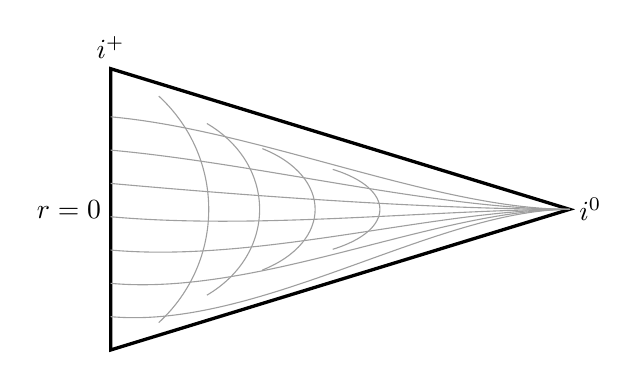
\begin{tikzpicture}[scale=0.94]
\coordinate (O) at (0,0);
\coordinate (P) at (0,3.8);
\coordinate (I) at (6.2,1.9);
\draw[very thick] (O)--(P)--(I)--cycle;
\foreach \y in {0.45,0.90,1.35,1.80,2.25,2.70,3.15} {
  \draw[gray!75] (0,\y) .. controls (2.0,\y-0.18) and (4.4,1.9) .. (I);
}
\draw[gray!75] (0.65,0.37) .. controls (1.55,1.20) and (1.55,2.60) .. (0.65,3.43);
\draw[gray!75] (1.30,0.74) .. controls (2.25,1.30) and (2.25,2.50) .. (1.30,3.06);
\draw[gray!75] (2.05,1.08) .. controls (3.00,1.46) and (3.00,2.34) .. (2.05,2.72);
\draw[gray!75] (3.00,1.36) .. controls (3.85,1.62) and (3.85,2.18) .. (3.00,2.44);
\node[left] at (0,1.9) {\(r=0\)};
\node[above] at (P) {\(i^+\)};
\node[right] at (I) {\(i^0\)};
\end{tikzpicture}
\caption{上半楔形區域的簡化圖。曲線是定性表示的等 \(r\) 與等 \(t\) 曲線族，並非精確的座標網格。}
\label{fig:l05-flat-wedge}
\end{figure}

固定 \(r\) 的世界線在緊緻化之前是垂直的，之後則彎曲，並在未來類時無窮遠附近逐漸密集。等 \(t\) 切片也同樣朝空間無窮遠處逐漸密集。這種密集是座標效應，不是物質真的受到物理壓縮。

\(45^\circ\) 規則直接適用於徑向光線。具有角動量的光線可能不會經過原點，而是在距原點非零的最近點折返，向外傳播。遠離原點時，它在圖上的投影看起來幾乎是徑向運動；只有接近最近點時，約化後的 \((t,r)\) 軌跡才會明顯彎曲。第一個工作部分到此完成。

\section{第二個工作部分：永恆史瓦西時空}

最大延拓的史瓦西解包含兩個外部菱形區域、一個未來黑洞區域，以及一個過去白洞區域。上下兩條波浪形邊界分別是未來奇點與過去奇點。由坍縮形成黑洞時，這個結構的大部分都會被捨棄；但我們需要的恰好是右側一般的外部區域。

\begin{figure}[htbp]
\centering
\includegraphics[width=0.72\textwidth]{lecture_05_figure_03.png}
\caption{永恆史瓦西圖；右側是一般的外部區域及其示意座標網格。}
\lectureframe{00:16:55.975}
\end{figure}

\begin{figure}[htbp]
\centering
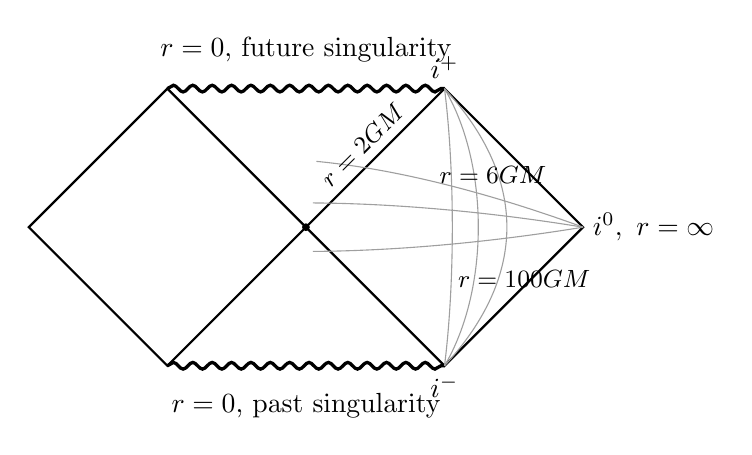
\begin{tikzpicture}[scale=0.88]
\coordinate (C) at (0,0);
\coordinate (TL) at (-2.0,2.0);
\coordinate (L) at (-4.0,0);
\coordinate (BL) at (-2.0,-2.0);
\coordinate (TR) at (2.0,2.0);
\coordinate (R) at (4.0,0);
\coordinate (BR) at (2.0,-2.0);
\draw[thick] (C)--(TL)--(L)--(BL)--(C);
\draw[thick] (C)--(TR)--(R)--(BR)--(C);
\draw[very thick,decorate,decoration={snake,amplitude=1.2pt,segment length=7pt}] (TL)--(TR);
\draw[very thick,decorate,decoration={snake,amplitude=1.2pt,segment length=7pt}] (BL)--(BR);
\draw[gray!75] (TR) .. controls (2.15,0.8) and (2.15,-0.8) .. (BR);
\draw[gray!75] (TR) .. controls (2.65,0.9) and (2.65,-0.9) .. (BR);
\draw[gray!75] (TR) .. controls (3.20,0.7) and (3.20,-0.7) .. (BR);
\draw[gray!75] (0.15,0.95) .. controls (1.5,0.82) and (2.9,0.40) .. (R);
\draw[gray!75] (0.10,0.35) .. controls (1.5,0.34) and (2.9,0.18) .. (R);
\draw[gray!75] (0.10,-0.35) .. controls (1.5,-0.34) and (2.9,-0.18) .. (R);
\fill (C) circle (1.6pt);
\node[above] at (TR) {\(i^+\)};
\node[below] at (BR) {\(i^-\)};
\node[right] at (R) {\(i^0,\ r=\infty\)};
\node[above] at (0,2.25) {\(r=0\), future singularity};
\node[below] at (0,-2.25) {\(r=0\), past singularity};
\node[rotate=45,above,font=\small] at (1.0,1.0) {\(r=2GM\)};
\node[font=\small] at (2.70,0.75) {\(r=6GM\)};
\node[font=\small] at (3.15,-0.75) {\(r=100GM\)};
\end{tikzpicture}
\caption{在大半徑處，右側外部區域看起來像平直楔形。當 \(c=1\) 時，它的內側零邊界是 \(r=2GM\)；其他標示的半徑則是示意例子。}
\label{fig:l05-eternal-schwarzschild}
\end{figure}

離黑洞越遠，外部區域就越像緊緻化的平直空間。像 \(r=6GM\) 和 \(r=100GM\) 這樣的線，逐漸呈現一般等半徑世界線的性質。外部區域的內側邊界位於
\begin{equation}
r=2GM
\end{equation}
單位制為 \(c=1\)。

接近中心時，就不能再拿平直空間來類比。閔可夫斯基時空中的徑向光線到達 \(r=0\) 後，會在物理空間的另一側重新出現。史瓦西時空內部中指向未來的光線不會反彈，而是終止於 \(r=0\) 處的類空奇點。坍縮的建構必須保留這項因果差異。

\section{讓我們得以拼接各部分的定理}

缺少的要素首先出現在牛頓重力學中。對球對稱的質量分布，高斯定律給出
\begin{equation}
\oint\mathbf g\cdot d\mathbf A=-4\pi G M_{\mathrm{enc}},
\end{equation}
因此
\begin{equation}
\mathbf g(r)=-\frac{G M_{\mathrm{enc}}(r)}{r^2}\,\hat{\mathbf r}.
\label{eq:l05-shell-theorem}
\end{equation}
半徑為 \(r\) 的球面外物質，在該處不會產生淨場。對總質量為 \(M\) 的空心球殼，
\begin{equation}
\mathbf g=
\begin{cases}
0, & r<R_{\mathrm{shell}},\\[3pt]
-\dfrac{GM}{r^2}\hat{\mathbf r}, & r>R_{\mathrm{shell}}.
\end{cases}
\end{equation}

伯克霍夫定理是相對論中的對應定理。每個球對稱真空區域，在局部上都是質量參數為常數的史瓦西區域。球殼內部的空區域，其質量參數為零，在局部上是閔可夫斯基時空；外部的質量參數為 \(M\)，是史瓦西時空：
\begin{equation}
\begin{aligned}
M_{\mathrm{enc}}&=0 && \text{inside the shell},\\
M_{\mathrm{enc}}&=M && \text{outside the shell}.
\end{aligned}
\label{eq:l05-birkhoff}
\end{equation}
即使球殼正在運動，這項敘述仍然適用，因為球殼兩側的真空區域仍保持球對稱。

\editorialnote{內部平直是一項局部敘述。靜態球殼即使不改變內部曲率，也可能改變內部時間座標的正規化。若球殼正在運動或為零類，兩側真空度規必須在球殼處匹配；這種理想化建構屬於薄殼接合，與入射 Vaidya 幾何密切相關。這些限制條件都不影響此處採用的因果剪接論證。}

若要想像實驗室中的情景，可以設想一個球面上密布同步雷射器，如大型慣性約束裝置中的雷射器，全部同時向內發射。在理想化模型中，沒有任何裝置，只有一個完美球形的光殼。殼層攜帶能量 \(E\)，因此外部質量參數為
\begin{equation}
M=\frac{E}{c^2},
\end{equation}
或者在自然單位制中簡寫為 \(E=M\)。球殼以光速傳播，所以在約化圖上是一條入射零線。這條線上的每一點都代表整個球形波前，而不是單一光子的軌跡。

\section{縫合坍縮時空}

從平直時空開始，畫出入射零殼層。殼層內部是正確的：伯克霍夫定理指出，這裡是平直時空。殼層外部則不對，因為外部幾何必須已反映出殼層的總質量，成為史瓦西幾何。

接著，在永恆史瓦西圖上畫出同一個殼層。這時殼層外部的區域是正確的。若坍縮從一般的空無一物狀態開始，白洞、另一個外部區域，以及黑洞內部不適用的部分都不對，因此把它們擦掉。

\begin{figure}[htbp]
\centering
\includegraphics[width=0.72\textwidth]{lecture_05_figure_05.png}
\caption{以紅色表示的零類殼層橫跨史瓦西圖；同時，正確的外部區域正被分離出來。}
\lectureframe{00:32:00.000}
\end{figure}

在平直時空部分，球殼抵達 \(r=0\)；在史瓦西時空部分，它抵達未來奇點的起始處。這是同一個端點。沿著殼層把平直內部與史瓦西外部接合，就得到描述黑洞形成的最簡單時空。

\begin{classroomqa}
\audiencequestion{在左上方的接合點，平直時空中的端點真的與史瓦西時空那一側的點相同嗎？\lecturetimestamp{00:34:50}}
\lecturerresponse{是的。平直時空中的殼層收縮至 \(r=0\)，史瓦西奇點也位於 \(r=0\)。這兩個被識別為同一點的位置，具有相同的幾何意義：二維球面已收縮至零大小。}
\end{classroomqa}

\begin{figure}[htbp]
\centering
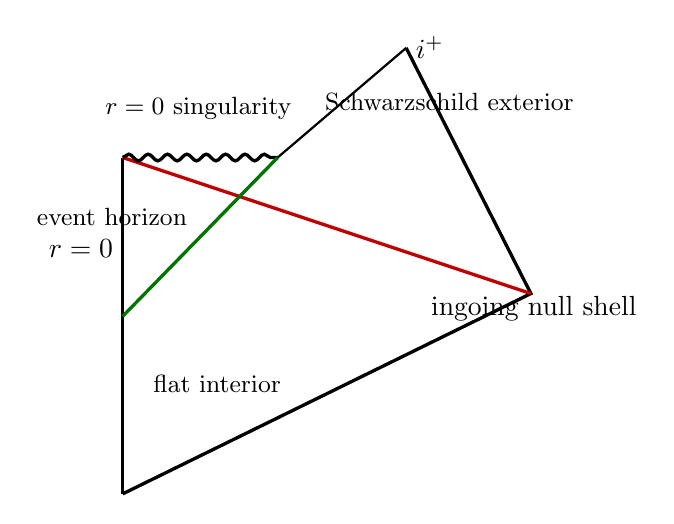
\begin{tikzpicture}[scale=0.96]
\coordinate (A) at (0,-2.8);
\coordinate (B) at (0,1.65);
\coordinate (C) at (2.05,1.65);
\coordinate (D) at (5.4,-0.15);
\coordinate (E) at (3.75,3.10);
\coordinate (H0) at (0,-0.45);
\draw[very thick] (A)--(B);
\draw[very thick] (A)--(D)--(E);
\draw[very thick,red!75!black] (D)--(B);
\draw[very thick,decorate,decoration={snake,amplitude=1.2pt,segment length=7pt}] (B)--(C);
\draw[very thick,green!45!black] (H0)--(C);
\draw[thick] (C)--(E);
\node[left] at (0,0.45) {\(r=0\)};
\node[below right] at (3.95,-0.05) {ingoing null shell};
\node[font=\small] at (1.25,-1.35) {flat interior};
\node[font=\small,anchor=west] at (2.55,2.38) {Schwarzschild exterior};
\node[above,font=\small] at (1.0,2.02) {\(r=0\) singularity};
\node[above left,font=\small] at (0.98,0.62) {event horizon};
\node[right] at (E) {\(i^+\)};
\end{tikzpicture}
\caption{坍縮幾何。紅色殼層將平直內部接合至史瓦西外部。綠色事件視界在平直區域中較早處開始，並終止於黑洞區域的未來邊界。}
\label{fig:l05-collapse}
\end{figure}

這項建構回答了永恆解留下的問題。由坍縮形成的黑洞沒有過去白洞，也沒有第二個漸近平坦宇宙，但仍有未來奇點。

\section{視界是一道全域邊界}

舊的標記 \(r=2GM\) 可以在穩態史瓦西幾何中標出視界，但它不是動態時空所需的定義。

\begin{definition}
未來事件視界是這樣一道邊界：它界定了所有能向未來零無窮遠傳送未來指向因果訊號的事件所構成的集合。
\end{definition}

在坍縮圖上，追蹤那條剛好無法逃逸的向外零射線。緊鄰它外側的射線會抵達無窮遠；緊鄰它內側的射線則終止於奇點。這條分界線就是真正的視界。

\begin{figure}[htbp]
\centering
\includegraphics[width=0.72\textwidth]{lecture_05_figure_06.png}
\caption{黑板上的建構完成。入射殼層以紅色表示，事件視界以綠色表示；部分綠線位於殼層下方仍然平直的區域。}
\lectureframe{00:39:10.000}
\end{figure}

現在這個令人驚訝的特徵已無法迴避。視界向過去延伸到殼層尚未抵達的區域。那裡的幾何在局部上是平直的；觀測者穿過那條線時，不會偵測到曲率脈衝、牆壁或閃光。然而，觀測者已無法抵達無窮遠，因為未來的殼層會封住所有可能的逃逸路徑。事件視界正是在這種全域意義上具有目的論性質：要定位事件視界，必須知道整個時空的未來。\editorialnote{沒有任何局部實驗能判定自己剛穿過一道平滑的事件視界。表觀視界或陷獲視界等其他概念較具局部性，在坍縮過程中不一定與事件視界重合。}

排水口的比喻凸顯了因果上的關鍵。想像一位划船者在平靜湖面上的塞住排水口附近。如果塞子永遠不拔，划船者就能離開；但如果確定有人會拔掉塞子，之後形成的水流可能使逃離變得不可能，即使眼下水面尚未流動。冰凍的尼加拉瀑布也說明同一點：水面平靜，不代表未來一定有通往安全之處的路。

\begin{classroomqa}
\audiencequestion{光的球殼越來越集中，所以塞子才被拔掉嗎？\lecturetimestamp{00:43:13}}
\lecturerresponse{這種集中會形成黑洞，但排水口的故事只用來說明較窄的一點：即使局部尚未發生任何戲劇性的變化，人也可能已經越過無法回頭的界線。}
\end{classroomqa}

\subsection{由增大的球面構成的視界}

約化圖上視界的每一點都代表一個 \(S^2\)。在視界的起點，該球面的面積為零。沿著視界向上移動，球面逐漸增大，直到面積半徑達到
\begin{equation}
R_s=\frac{2GM}{c^2}.
\end{equation}
對於穩態黑洞，它會維持在這個大小；若有更多能量落入，球面就會再度增大。

\editorialnote{在理想化的球對稱坍縮圖中，視界生成元在 \(r=0\) 上的一個形成點，也就是摺痕處相交。面積為零的是這個極限二維球面；這不應解讀成有限大小的史瓦西視界突然縮成一點。}

\subsection{遠方觀測者能重建什麼}

接下來較長的討論，會把已在全域視界內的觀測者，與該觀測者如何來到那裡的歷史分開處理。

\begin{classroomqa}
\audiencequestion{殼層抵達之前，被困住的人處於什麼狀態？從遠方觀測者的角度來看，那個人是否在視界之外？\lecturetimestamp{00:44:03}}
\lecturerresponse{不是。一旦世界線進入事件視界之內，它的未來就會抵達奇點，而它再也無法傳送新訊號給遠方觀測者。不過，那個人並不是從那裡才開始存在。更早的粒子、祖先或其他前身能量，都是從可被觀測的區域進入的。}
\end{classroomqa}

因此，遠方觀測者可能看見前身物質接近視界，卻始終收不到來自視界內部的訊號。能看穿入射殼層並不矛盾：殼層由光構成，觀測者也能看見殼層本身，並推知黑洞已經形成。

\begin{classroomqa}
\audiencequestion{視線會穿過坍縮中的殼層嗎？外部觀測者仍然能知道黑洞已形成嗎？\lecturetimestamp{00:46:51}}
\lecturerresponse{能。觀測者看得到入射殼層，也能收到路徑穿過殼層、且仍能逃逸的光。令人覺得奇怪的是，前身物質在殼層抵達中心之前，就已接近剛被確定的視界。}
\end{classroomqa}

\begin{classroomqa}
\audiencequestion{這是否延續了那項規則：從外部看，物質似乎被壓縮到視界上？\lecturetimestamp{00:47:49}}
\lecturerresponse{是。在外部的描述中，物質仍與視界相連，並且持續紅移，直到後來黑洞蒸發的量子過程改變這個圖景。}
\end{classroomqa}

這種外部描述引出下一個主題。如果資訊看似塗布在二維表面上，那麼黑洞熵隨表面積變化也就不那麼令人意外。

\section{從無窮遠處觀測到的熵與溫度}

在大型視界附近，可以用局部平面取代球面，就像在小型實驗室裡採用平地近似一樣。這時可以將前面討論的兩項事實放在一起：
\begin{equation}
\begin{aligned}
S_{\mathrm{BH}}&\propto A_H,\\
\Delta A_H&\sim \ell_P^2
\quad\text{per added bit, schematically}.
\end{aligned}
\end{equation}
「每個普朗克面積對應一個位元」這個助記說法表達的是面積律，並不是微觀推導。

在遠離史瓦西黑洞處測得的霍金溫度為
\begin{equation}
T_H=\frac{\hbar c^3}{8\pi GMk_B}.
\label{eq:l05-hawking}
\end{equation}
代入 \(R_s=2GM/c^2\)，可得
\begin{equation}
T_H=\frac{\hbar c}{4\pi k_B R_s}.
\label{eq:l05-hawking-radius}
\end{equation}
因此，黑洞越大，溫度越低。

\begin{classroomqa}
\audiencequestion{溫度會隨位置改變嗎？\lecturetimestamp{00:52:43}}
\lecturerresponse{日常談話中，答案顯然是會：紐約和史丹佛的溫度不必相同。更精確的問題是：在引力熱平衡的系統中，情況如何？在這種系統裡，即使經過紅移的平衡溫度維持不變，不同高度的局部溫度計讀數仍可能不同。}
\end{classroomqa}

溫度是透過局部動能讀取的。在受熱地球上方的稀薄大氣中，分子上升時動能減少，下降時動能增加。光子向上傳播時紅移，向下傳播時藍移。因此，高處與低處的溫度計讀數不一定對應相同的局部能量尺度。

對靜態時空，平衡關係為
\begin{equation}
T_{\mathrm{loc}}(r)\sqrt{-g_{tt}(r)}=T_\infty,
\label{eq:l05-tolman}
\end{equation}
這就是托爾曼定律。方程~\eqref{eq:l05-hawking}中的霍金溫度是 \(T_\infty\)，也就是在無窮遠處正規化後的讀數。

\section{視界附近的高溫靜態大氣}

令 \(\rho\) 表示從視界向外量測的固有距離。在大型史瓦西黑洞的視界附近，方程~\eqref{eq:l05-tolman}可化為
\begin{equation}
k_B T_{\mathrm{loc}}(\rho)
\simeq\frac{\hbar c}{2\pi\rho},
\label{eq:l05-local-temperature-si}
\end{equation}
或者以 \(c=\hbar=k_B=1\) 為單位，寫成
\begin{equation}
T_{\mathrm{loc}}(\rho)=\frac{1}{2\pi\rho}.
\label{eq:l05-local-temperature}
\end{equation}

\begin{figure}[htbp]
\centering
\includegraphics[width=0.72\textwidth]{lecture_05_figure_07.png}
\caption{黑板上標示的漸近霍金溫度與近視界局部溫度 \(T(\rho)=1/(2\pi\rho)\)。}
\lectureframe{01:02:40.000}
\end{figure}

用纜線固定在 \(\rho\) 處的小型溫度計，會隨著下降而測得越來越高的溫度。維持在這種靜態大氣中的原子會先受激，接著電離，然後解離；局部能量再升高時，連原子核和強子也無法保持完整。若讓人腳朝下下降，會得到令人難忘的診斷：腳會很燙。

\emph{固定}一詞至關重要。這種發散只會出現在靠加速維持靜止的探測器上。它描述的是相對於外部時間發生紅移的熱大氣。自由落下的探測器沿著不同軌跡運動；對處於規則量子態中的大型黑洞而言，探測器不一定會在視界處遇到發散的熱浴。\editorialnote{這項區分，將靜止觀測者測得的托爾曼溫度與加速度溫度，和自由落下觀測者的規則局部經驗區別開來。講課刻意把這項對照轉化為一個操作上的疑問，而不只靠術語來消解。}

電離閾值讓這項衝突變得具體。

\begin{classroomqa}
\audiencequestion{氫原子電離需要多少能量？\lecturetimestamp{01:06:53}}
\lecturerresponse{課堂上給出的答案是 \(13\) 電子伏特，正確指出了基態電離能為 \(13.6\,\mathrm{eV}\)。附帶估算的數千開爾文太低了，但這項論證只需要存在有限的電離閾值。}
\end{classroomqa}

確實，
\begin{equation}
\frac{13.6\,\mathrm{eV}}{k_B}\simeq1.58\times10^5\,\mathrm{K}.
\end{equation}
因此，在某個小的固有距離 \(\rho_{\mathrm{ion}}\) 處，靜態溫度會達到電離尺度。靜態外推表示，原子在那裡、也就是視界之外，就應該已經電離。相較之下，自由落下的原子預期不會遇到局部的牆，而且能在有限固有時間內穿過視界。外部觀測者能否做一項實驗，判定這兩種描述何者成立？

\section{海森堡顯微鏡}

先回想光子顯微鏡，再把這個問題應用到黑洞。要以解析度 \(\Delta x\) 定位粒子，探測光的波長必須滿足
\begin{equation}
\lambda\lesssim\Delta x.
\end{equation}
因此，一個光子至少帶有以下動量：
\begin{equation}
p_\gamma\gtrsim\frac{\hbar}{\Delta x}.
\label{eq:l05-microscope}
\end{equation}
散射這個光子會造成同一量級的反衝。若先量測位置，緊接著再檢查速度，第二次量測所見的狀態已被第一次量測改變。這項實驗反而製造了原本想排除的狀況。

\begin{figure}[htbp]
\centering
\includegraphics[width=0.70\textwidth]{lecture_05_figure_08.png}
\caption{顯微鏡的估算給出 \(\Delta x\gtrsim\lambda\) 與 \(p_\gamma\gtrsim\hbar/\Delta x\)。}
\lectureframe{01:11:50.000}
\end{figure}

這不只是古典光學的限制。古典波可以任意微弱；量子力學則要求成功探測時至少有一個量子。因此，提高空間解析度必然需要有限的動量轉移。

\section{近視界實驗}

現在讓一個原子穿越從 \(\rho_{\mathrm{ion}}\) 開始的區域。相對於靜止參考系，它正以接近 \(c\) 的速度向內運動，因此在穿越視界前可用的時間間隔約為
\begin{equation}
\Delta\tau\sim\frac{\rho_{\mathrm{ion}}}{c}.
\label{eq:l05-fall-time}
\end{equation}
穿越視界後，任何結果都無法傳回外部。測量必須在這段短時間內分辨出原子是否完好，或已經電離。

要在這個區域內解析出原子，必須滿足
\begin{equation}
\lambda\lesssim\rho_{\mathrm{ion}}.
\end{equation}
因此，探測能量至少受限於
\begin{equation}
E_\gamma=cp_\gamma
\gtrsim\frac{\hbar c}{\rho_{\mathrm{ion}}}.
\label{eq:l05-probe-energy}
\end{equation}
除了因子 \(2\pi\) 之外，這和方程~\eqref{eq:l05-local-temperature-si}所示的是同一個尺度：
\begin{equation}
E_\gamma\gtrsim2\pi k_B T_{\mathrm{loc}}(\rho_{\mathrm{ion}}).
\label{eq:l05-probe-temperature}
\end{equation}
足以解析事件的光子，也有足夠能量電離原子。

\begin{figure}[htbp]
\centering
\includegraphics[width=0.72\textwidth]{lecture_05_figure_09.png}
\caption{黑板上的近視界估算：\(\lambda<\rho\) 要求局部探測能量達到 \(\hbar c/\rho\) 的量級。}
\lectureframe{01:18:30.000}
\end{figure}

\begin{classroomqa}
\audiencequestion{這個高能光子在原子自己的自由落下參考系中，也會使原子電離嗎？\lecturetimestamp{01:19:07}}
\lecturerresponse{會。原子會受到一個真實的高能量子撞擊，並在自己的局部參考系中反衝或電離。這項測量呈現的不是毫無干擾的下落；測量本身改變了下落狀態。}
\end{classroomqa}

\begin{classroomqa}
\audiencequestion{如果原子只是自由落下，沒有人做這項實驗呢？\lecturetimestamp{01:19:39}}
\lecturerresponse{那麼就不會發生這種特定的擾動。若外部觀測者真的進行高解析度實驗，原子就會陷入困境。這項論證探討的是外部能驗證什麼，並不是要證明未受測量的落入者會被燒灼。}
\end{classroomqa}

\subsection{溫度計或發射器能不能做得更好？}

移動儀器並不能解決資訊問題。

\begin{classroomqa}
\audiencequestion{能否在較遠處量測、推斷溫度梯度，或讓自由落下的溫度計記錄溫度，之後再取回紀錄？\lecturetimestamp{01:19:51}}
\lecturerresponse{要取得近視界的紀錄，就必須有某種東西與溫度計作用，再以量子的形式把資訊傳回。讓溫度計掉頭需要劇烈加速；遠端讀取則需要發射或散射。無論採取哪種方式，都會改變原本要檢驗其未受干擾歷史的物理系統。}
\end{classroomqa}

\begin{classroomqa}
\audiencequestion{為了達到更高解析度而需要高探測能量，和把反射觀測從近視界區域傳出去，是否是同一個難題？\lecturetimestamp{01:21:51}}
\lecturerresponse{兩者是同一紅移尺度的兩面。光子最後抵達無窮遠時，能量可能很低，因為它在向外傳播時損失了能量；但在解析原子的地方，它必須具有很高的局部頻率。}
\end{classroomqa}

\editorialnote{在視界外不遠處發出的光子，光是要逃離視界，並不需要有很高能量。這裡的關鍵條件是，必須在固有時間與距離都約為 \(\rho\) 的尺度內記錄下事件；接著，引力紅移會把很高的局部頻率對應到小得多的漸近頻率。}

\begin{classroomqa}
\audiencequestion{物體能不能自行發出資訊，而不必受外部光子撞擊？\lecturetimestamp{01:22:51}}
\lecturerresponse{可以，但局部發射仍須具備足夠頻寬，才能辨識短時間內發生了什麼。發射也會使物體反衝。用發射器取代反射光，並不能免費留下紀錄。}
\end{classroomqa}

\begin{classroomqa}
\audiencequestion{下落的原子有一個偏好的方向。這種有方向性的動能也稱為溫度嗎？\lecturetimestamp{01:23:10}}
\lecturerresponse{不是。把棒球丟出去，不會讓棒球變熱。整體下落能量與熱擾動是兩回事。論證中的溫度屬於周圍靜態的輻射大氣，與原子的質心運動無關。}
\end{classroomqa}

\begin{classroomqa}
\audiencequestion{共同下落的實驗室能用磁場檢驗原子是否已電離嗎？\lecturetimestamp{01:23:50}}
\lecturerresponse{實驗室可以在局部進行檢驗。難處在於，必須在穿越視界之前把結果傳回外部。這種通訊同樣需要相互作用，以及具備所需局部解析度的出射量子。}
\end{classroomqa}

\begin{classroomqa}
\audiencequestion{如果把發射器裝在溫度計裡，它所需的局部能量會不會太高，以致摧毀儀器？\lecturetimestamp{01:24:57}}
\lecturerresponse{這就是同一個障礙在工程上的表現。愈接近視界，在相關的局部尺度上，訊號所需的能量就愈接近待檢驗的熱能尺度。}
\end{classroomqa}

\begin{classroomqa}
\audiencequestion{高溫區域是否薄到讓人來不及從容完成測量？\lecturetimestamp{01:25:15}}
\lecturerresponse{正是如此。其固有厚度約為\(\rho\)，穿越時間約為\(\rho/c\)。這項限制可以描述為空間解析度不足，也可以描述為時間頻寬有限；無論如何描述，都需要高局部動量或能量。}
\end{classroomqa}

相應的時間頻寬估計式為
\begin{equation}
\Delta E\,\Delta\tau\gtrsim\hbar.
\end{equation}
這裡應將它理解為傅立葉解析度或操作上的解析度界限，而不是與\(\Delta x\,\Delta p\geq\hbar/2\)地位相同的算符不確定性關係。講座以啟發式方式援引時間能量不確定性；由空間解析度推導出的方程~\eqref{eq:l05-probe-energy}才是論證中較為確鑿的部分。

\begin{classroomqa}
\audiencequestion{能否用較低能量、較低解析度的探針測量許多原子，再以統計方式得到答案？\lecturetimestamp{01:26:26}}
\lecturerresponse{這是個合理的問題，講座中沒有給出定論。每個原子只有一次通過的機會，而要從訊號中還原答案，仍須有足夠資訊辨認短暫的近視界事件。講座援引了不確定性原理，但沒有提出完整的統計不可行性證明。}
\end{classroomqa}

\enlargethispage{2\baselineskip}
\section{已確立與尚未確立的內容}

這項論證並未預言自由落下者必定會感受到發散的靜態溫度。

\begin{classroomqa}
\audiencequestion{我們是在說，可以預言下落者不會感受到這種溫度嗎？\lecturetimestamp{01:27:38}}
\lecturerresponse{不是。結論的範圍較窄：若要透過外部實驗確認原子沒有經歷高溫擾動，實驗本身就會造成同一尺度的擾動。這就是這項操作分析所確立的全部內容。}
\end{classroomqa}

因此，這個結論既不是防火牆定理，也不是下落者會被燒傷的證明，更不是什麼都不會發生的證明。它限制的是外部驗證：\emph{要解析未受擾動的近視界事件，就需要一個會擾動該事件的探針}。
若進行實驗，實驗中的量子就會產生原本要檢驗的效應。若不進行實驗，單憑這項論證並不能確立任何額外且可由實驗取得的事實。這裡刻意拿雙狹縫實驗作類比：未測量路徑就追問粒子通過哪條狹縫，以及沒有相互作用就追問外部裝置能證實什麼，都是試圖在無法取得所需證據的情況下，仍要給出操作上的答案。